\documentclass[a4paper]{article}
\usepackage{times}
\usepackage[utf8]{inputenc}
\usepackage[T1]{fontenc}
\usepackage{graphicx}
\usepackage{amssymb}
\usepackage{hyperref}
\linespread{1.5}	% double spaces lines
\usepackage[hmargin=3cm,vmargin=3cm]{geometry}
\usepackage{indentfirst}
\usepackage[fleqn]{amsmath}
\usepackage{amsthm}
\usepackage{sectsty}
\usepackage{enumitem}
\usepackage[brazil]{babel}
\usepackage{placeins} %mantem figuras na secao com \FloatBarrier
\usepackage{fixltx2e} %\textsubscript
\usepackage{textcomp}
\hypersetup{%
    pdfborder = {0 0 0}
}
\sectionfont{\normalsize}
\subsectionfont{\small}
\begin{document}

\begin{center}


\large{ 
\uppercase{ Universidade Federal do Rio Grande do Sul\\

Instituto de Informática \\

Curso de Ciência da Computação \\

Teoria da Computação N (2014/1)\\
}

Prof. Dr. Tiarajú Asmuz Diverio \\


Graduandos: \\ Paulo Renato Lanzarin, Ricardo Gabriel Herdt e \\
	Wladimir Leuschner \\[1.5cm]



% Title
\LARGE {\bfseries Simulação de exemplos de Cálculo Lambda \\[1.0cm]
}}

\end{center}

\section*{Exemplo 8.9c)}

$\mathbf{x\ \lambda x.\lambda y.(x\ y)}$

\begin{figure}[h]
  \centering
  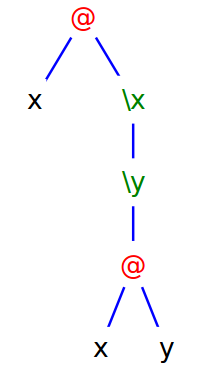
\includegraphics[scale=0.5]{8-9e.png}
  \caption{Exemplo 8.9c}
\end{figure}

\FloatBarrier

\section*{Exemplo 8.10f)}

$\mathbf{((\lambda p.p\ (p\ q))\ (\lambda r.(p\ r)))}$

\begin{figure}[h]
  \centering
  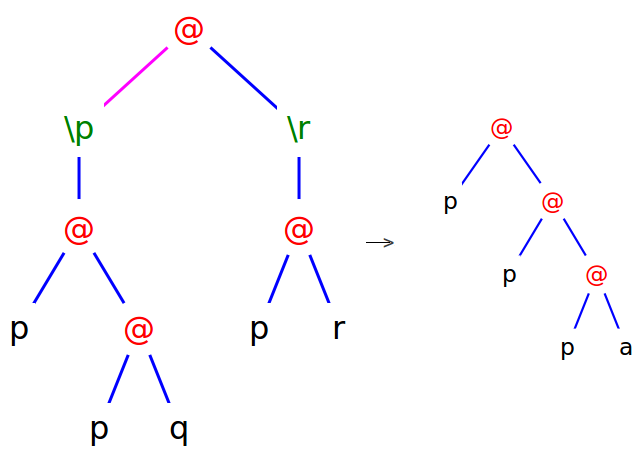
\includegraphics[scale=0.5]{8-10f.png}
  \caption{Exemplo 8.10f antes e após a substituição}
\end{figure}

\FloatBarrier

\section*{Exemplo 8.11}
\subsection*{a)}
$\mathbf{(\lambda x.2 * x + 1)\ 3\ \rhd (2 * x + 1) [x \leftarrow 3] = 2*3 + 1 = 7}$

\begin{figure}[h]
  \centering
  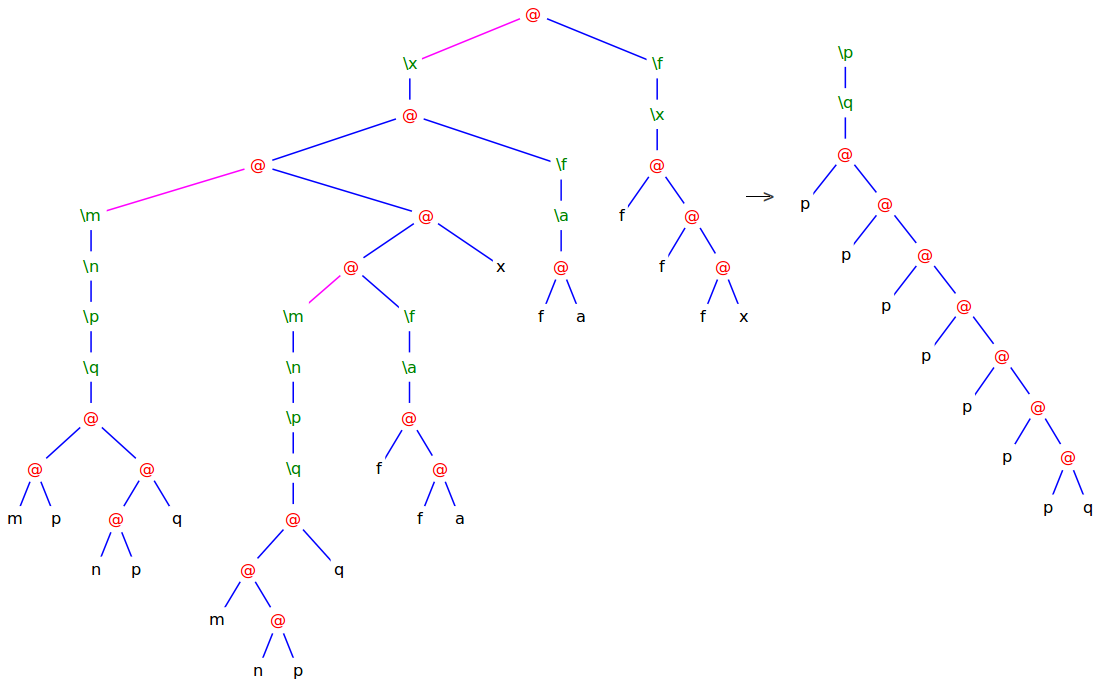
\includegraphics[scale=0.5]{8-11a_1.png}
  \caption{Exemplo 8.11a antes e após ser reduzido}
\end{figure}

\FloatBarrier
\subsection*{b)}
\begin{align*}
\mathbf{(\lambda x.\lambda y.x + y)\ 5\ \rhd }\\
\mathbf{(\lambda y.x + y) [x \leftarrow 5]}
\end{align*}

\begin{figure}[h]
  \centering
  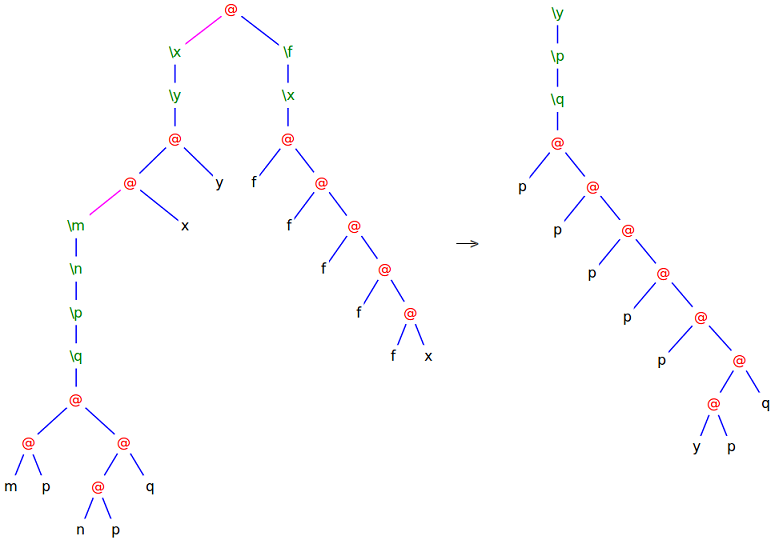
\includegraphics[scale=0.5]{8-11_b.png}
  \caption{Exemplo 8.11b antes e após ser reduzido}
\end{figure}

\FloatBarrier

\subsection*{c)}

\begin{figure}[h]
  \centering
  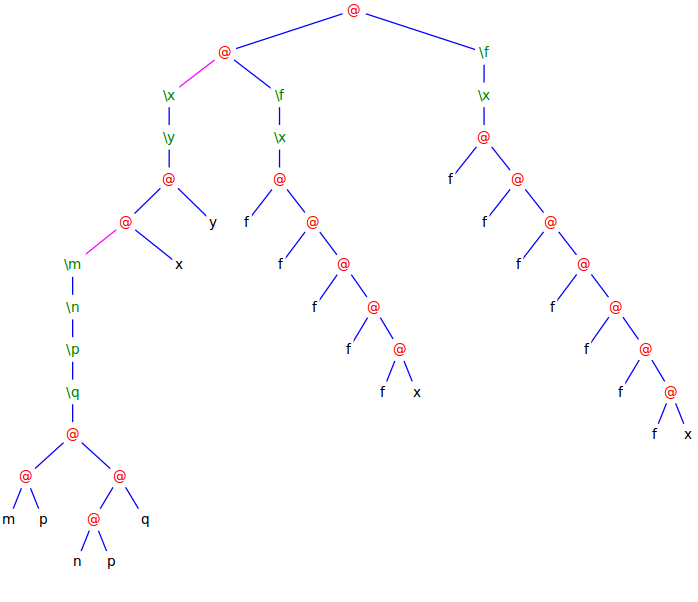
\includegraphics[scale=0.5]{8-11c_1.png}
  \caption{Exemplo 8.11c antes de ser reduzido}
\end{figure}

\begin{figure}[h]
  \centering
  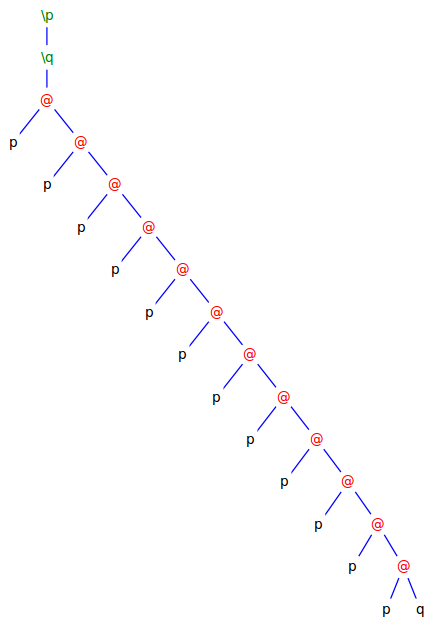
\includegraphics[scale=0.5]{8-11c_2.png}
  \caption{Exemplo 8.11c após ser reduzido}
\end{figure}

\FloatBarrier

\subsection*{d)}


\FloatBarrier

\subsection*{f)}

\begin{figure}[h]
  \centering
  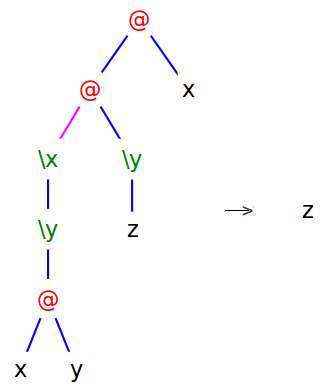
\includegraphics[scale=0.5]{8-11f.png}
  \caption{Exemplo 8.11f antes e após ser reduzido}
\end{figure}

\FloatBarrier

\subsection*{g)}

\begin{figure}[h]
  \centering
  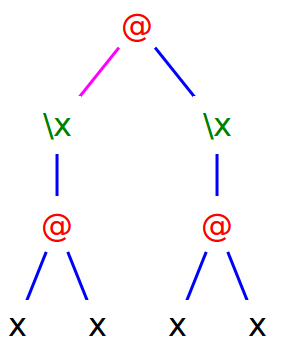
\includegraphics[scale=0.4]{8-11g.png}
  \caption{Exemplo 8.11g antes e após ser reduzido}
\end{figure}

\FloatBarrier

\subsection*{h)}

\begin{figure}[h]
  \centering
  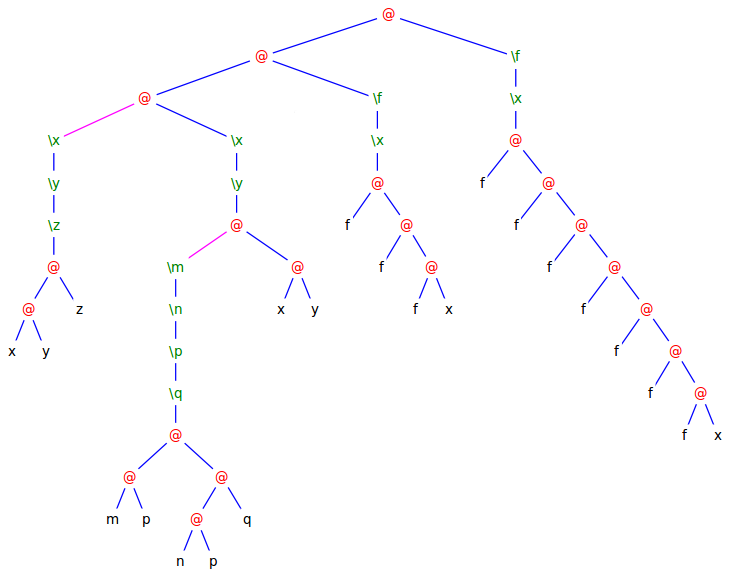
\includegraphics[scale=0.5]{8-11h_1.png}
  \caption{Exemplo 8.11h antes de ser reduzido}
\end{figure}

\begin{figure}[h]
  \centering
  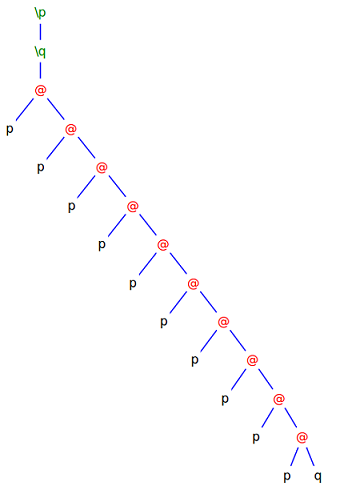
\includegraphics[scale=0.5]{8-11h_2.png}
  \caption{Exemplo 8.11h após  ser reduzido}
\end{figure}

\FloatBarrier


\end{document}
